Em colisões íons pesados(íons de chumbo ou ouro) a uma energia da ordem de $100 GeV$,
como na Figura \ref{qgp},é possível realizar a quebra momentânea dos hádrons constituintes desses núcleos, liberando novos graus
de liberdade para o movimento dos quarks, dessa maneira, atinge-se um novo estado da matéria, chamado Plasma de Quarks e Gluons,
ou QGP\footnote{Sigla em inglês para Plasma de Quarks e Gluons}. A temperatura necessária para formar este estado da matéria é da
ordem de milhares de $MeV$ ou $10^{10} K$, e a densidade de energia é da ordem de $0.2-1 GeV/fm^{3}$. As propriedades deste estado
da matéria podem ser estudadas analisando os produtos dessa colisão após o resfriamento da matéria. Através espectro de
$p_T$\footnote{Ver Apêndice \ref{variaveis}} das partículas, por exemplo, fornece insformações sobre a entropia e a temperatura do
plasma, através da multiplicidade e da inclinação do gráfico, respectivamente. Em geral, essas propriedades, referentes à expansão
hidrodinâmica do plasma\footnote{Ver Apêndice \ref{hidrodinamica}} estarão associados ao espectro na faixa de $p_T \approx 0-2 GeV/c$.
Na faixa $p_T > 2 GeV/c$, observa-se os efeitos de fenômenos da classe {\it hard scaterring}. Essas propriedadess são resultados da formação
de partículas de alta energia que atravessam o plasma aquecido, depositando energia neste. Na sua saída, devido às propriedades\footnote{Para
mais detalhes sobre as propriedades citadas, ver \cite{skands_introduction_2013}} da QCD\footnote{QCD ou {\it Quantum Chromodynamics}
é a teoria que descreve as interações fortes.}, essas partículas se fragmentam criando os chamados jatos ou {\it jets}\footnote{Para
uma definição mais precisa de jatos, ver Apêndice \ref{algoritmos}}. Esses jatos sofrem efeitos estruturais por conta da interação dos
partons iniciais\cite{lokhtin_angular_1998,bass_systematic_2009,connors_review_2017,nattrass_jet_2018,denterria_jet_2009} com o plasma.

%\begin{figure}[!h]


 \centering
 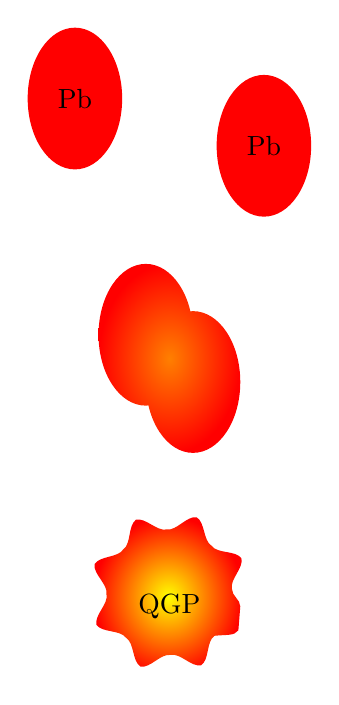
\begin{tikzpicture}[thick,scale=.3]

\fill[red] (0,23) ellipse (2 and 3) node [black,scale=1] {Pb};

\fill[red] (8,21) ellipse (2 and 3) node [black,scale=1] {Pb};

\shade[outer color=red,inner color=orange] (3,13) ellipse (2 and 3) -- (5,11) ellipse (2 and 3);

\shade[inner color=yellow, outer color=red,decorate,decoration={snake,amplitude=3,segment length=20}] (4,1.5) circle (3) node [scale=1] {QGP};

\end{tikzpicture}
\caption{Sequência temporal de colisão de íons pesados.}
\label{qgp}
\end{figure}

\begin{figure}[!h]
 \centering
 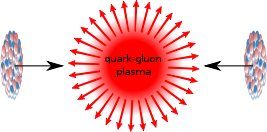
\includegraphics[scale=1]{Content/qgp.png}
 \caption{Colisão de núclos pesados, resultando na formação do Plasma de Quarks e Gluons.}
 \label{qgp}
\end{figure}


Assim como a perda de energia de jatos, ou \emph{jet quenching}, outros efeitos são considerados como assinaturas do Plasma de Quarks e Gluons,
tal como o aumento da produção de estranheza e a supressão de produção do $J/\Psi$ em relação às colisões $pp$. A produção de estranheza é uma assinatura que provém do
equilíbrio químico(ver \cite{letessier_hadrons_2002}) supostamente gerado no início da colisão. Esse aumento da produção de estranheza, ou \emph{strange production enhancement},
foi observado, em comparação com colisões p-p ou p-Pb, e pode ser observado na Figura \ref{strangeness}.

\begin{figure}
 \centering
 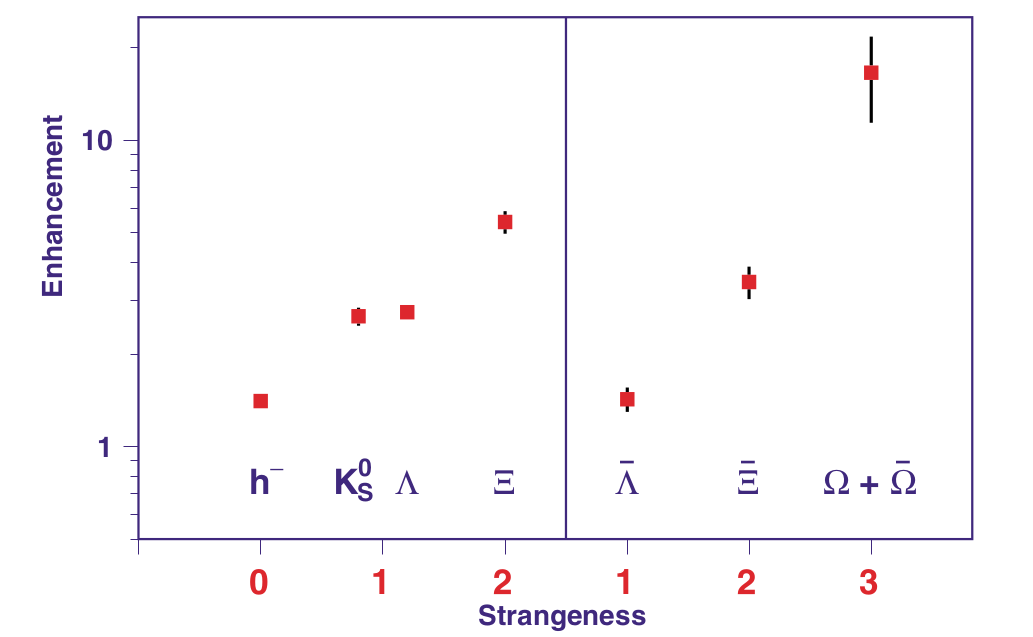
\includegraphics[scale=.3]{Content/strangeness.png}
 \caption{Aumento da produção de estranheza. O aumento é definido pela razão entre o número de contagens em colisões Pb-Pb e as contagens em p-Be. Resultados obtidos pelo experimento
 CERN WA97.}
 \label{strangeness}
\end{figure}